\documentclass[dvipdfmx,17pt]{beamer}

\usepackage{pxjahyper}
\usepackage{minijs}
\usepackage{amsthm}
\usepackage[all]{xy}


%\renewcommand{\subset}{\subseteq}
\renewcommand{\emptyset}{\varnothing}

\usefonttheme{professionalfonts}
\mathversion{bold}
\renewcommand{\kanjifamilydefault}{\gtdefault}
%\usetheme{Antibes}
\setbeamertemplate{navigation symbols}{}

%\setbeamertemplate{theorems}[numbered]
\setbeamertemplate{footline}[frame number] 


\theoremstyle{plain}
\newtheorem{thm}{定理}
\newtheorem{defi}[thm]{定義}
\newtheorem{lem}[thm]{補題}
\newtheorem{prop}[thm]{命題}
\newtheorem{cor}[thm]{系}
\renewcommand{\proofname}{証明}

\newcommand{\Z}{\mathbb{Z}}
\newcommand{\Q}{\mathbb{Q}}
\newcommand{\R}{\mathbb{R}}
\newcommand{\C}{\mathbb{C}}


\DeclareMathOperator{\Type}{type}

\title{ガロア理論と正$n$角形の作図}
\date{July 16, 2016}

\begin{document}

\begin{frame}\frametitle{}
\titlepage
\end{frame}

\begin{frame}
\begin{defi}[体]
四則演算$+, -, \times, \div$で閉じた集合$K$のことを体という.
\end{defi}
\end{frame}

\begin{frame}
例. $\Q, \R, \C$は体.
\end{frame}

\begin{frame}
体$K, L$について$K \subset L$であるとき,$L$は$K$の拡大体であるという.

これを$L/K$が体の拡大であるという.
\end{frame}

\begin{frame}
\begin{defi}
$L$を$K$の拡大体,$\alpha \in L$とする.
$K$を含み$\alpha$を持つ体のうち最小のものを$K$に$\alpha$を添加した体といい,$K(\alpha)$と書く.
\end{defi}
\end{frame}

\begin{frame}
例. $\Q$に$\sqrt{2}$を添加した体は
\[\Q(\sqrt{2}) = \{a+b\sqrt{2} | a, b \in \Q \} \]
である.
\end{frame}

\begin{frame}{ガロア理論とは}
ざっくり言えば「体の拡大を群を使って調べる」という理論である
\end{frame}

\begin{frame}{ガロア理論とは}
\begin{itemize}
\item 2次方程式,3次方程式,4次方程式には解の公式が存在する
\item 3次,4次の公式は15世紀に見つけられた.
\item 一方,5次方程式は一般に解けないことがアーベルによって証明された (1824年)
\item ここで方程式が解けるとは四則演算とべき根のみによって解を表せるということ
\end{itemize}
\end{frame}

\begin{frame}
\begin{itemize}
\item ガロアは与えられた代数方程式が解けるかどうかの必要十分条件を与えた (1832年).
\item そこで使われた理論を整備したものがガロア理論である.
\end{itemize}
\end{frame}

\begin{frame}
(注意:これからガロア理論に関する定義と定理の羅列が続きます.)
\end{frame}

\begin{frame}
体の拡大を調べる上でもっとも基本的であるのが,線形代数を使うこと

$L/K$が体の拡大であるとき,$L$を$K$上のベクトル空間とみることができる.
このとき$\dim_K L$を$L/K$の拡大次数といい,$[L:K]$と書く.
\end{frame}

\begin{frame}
例. $\Q$上のベクトル空間$\Q(\sqrt{2})$の基底として$\{1, \sqrt{2}\}$がとれる.よって
\[ [\Q(\sqrt{2}):\Q] = \dim_\Q \Q(\sqrt{2}) = 2 \]
\end{frame}

\begin{frame}
\begin{prop}[拡大次数の積の法則]
$L/M$, $M/K$がともに有限次拡大のとき$L/K$も有限次拡大で,
\[ [L:K] = [L:M][M:K]. \]
\end{prop}
\end{frame}

\begin{frame}
\begin{defi}
$L/K$を体の拡大,$\alpha \in L$とする.

$\alpha \in L$が$K$上代数的 $\overset{\mathrm{def}}{\iff}$ ある$K$係数多項式$f(x)$が存在して$f(\alpha) = 0$

$L/K$が代数拡大 $\overset{\mathrm{def}}{\iff}$ すべての$\alpha \in L$に対して$\alpha$は$K$上代数的.
\end{defi}
\end{frame}

\begin{frame}
\begin{defi}
$\alpha$が$K$上代数的であるとき,$K$係数多項式$f(x)$で$f(\alpha) = 0$となるもののうち次数が最小なものを$\alpha$の$K$上の最小多項式という.
\end{defi}
\end{frame}

\begin{frame}
\begin{thm}
$\alpha$の$K$の最小多項式を$f(x)$とするとき,
\[ [K(\alpha) : K] = \deg f(x) \]
\end{thm}
\end{frame}

\begin{frame}
例. $\sqrt{2}$の$\Q$上の最小多項式は$x^2-2$で次数は$2$.$[\Q(\sqrt{2}):\Q]$に一致.

$\sqrt[3]{2}$の$\Q$上の最小多項式は$x^3-2$で次数は$3$.よって$[\Q(\sqrt[3]{2}):\Q] = 3$.
\end{frame}

\begin{frame}
\begin{defi}[共役]
$\alpha$の$K$上の最小多項式を$f(x)$とする.このとき$f(x)$の根のことを$\alpha$の$K$上の共役という.
\end{defi}
\end{frame}

\begin{frame}
例.
\begin{itemize}
\item $\sqrt{2}$の最小多項式$x^2-2$の根は$\sqrt{2}, -\sqrt{2}$.
よって$\sqrt{2}$の$\Q$上の共役は$\sqrt{2}$と$-\sqrt{2}$.
\item $\sqrt[3]{2}$の最小多項式$x^3-2$の根は$\sqrt[3]{2}, \sqrt[3]{2}\omega, \sqrt[3]{2}\omega^2$.
よって$\sqrt[3]{2}$の$\Q$上の共役は$\sqrt[3]{2}, \sqrt[3]{2}\omega, \sqrt[3]{2}\omega^2$.
\end{itemize}
\end{frame}

\begin{frame}
\begin{defi}[ガロア拡大]
代数拡大$L/K$がガロア拡大 $\overset{\mathrm{def}}{\iff}$ 任意の$\alpha \in L$に対して$\alpha$の$K$上の共役はすべて$L$に属する.

{\small 本当は分離拡大という条件を考えないといけないがここでは正確さを犠牲にする}
\end{defi}
\end{frame}

\begin{frame}
\begin{itemize}
\item $\Q(\sqrt{2})/\Q$はガロア拡大
\item $\Q(\sqrt[3]{2})/\Q$はガロア拡大ではない.実際$\sqrt[3]{2}$の共役$\sqrt[3]{2} \omega$が$\Q(\sqrt[3]{2})$に入っていない.
\end{itemize}
\end{frame}

\begin{frame}
\begin{defi}[ガロア群]
$L$から$L$への全単射$\sigma$で次の条件をみたすもの全体を$\mathrm{Gal}(L/K)$と書き,$L/K$のガロア群という.
\begin{enumerate}
\item $\forall a \in K, \sigma(a) = a$
\item $\forall a, b \in L, \sigma(a+b) = \sigma(a) + \sigma(b)$
\item $\forall a, b \in L, \sigma(ab) = \sigma(a)  \sigma(b)$
\end{enumerate}
\end{defi}
\end{frame}

\begin{frame}
\begin{prop}
$\sigma \in \mathrm{Gal}(L/K), \alpha \in L$を$K$上代数的な元とする.
このとき$\sigma(\alpha)$は$\alpha$の$K$上の共役である
\end{prop}
\end{frame}

\begin{frame}
\begin{prop}
$L = K(\alpha)$のとき,$\mathrm{Gal}(L/K)$の元は$\alpha$の行き先だけで決まる.
\end{prop}
\end{frame}

\begin{frame}
例. $\mathrm{Gal}(\Q(\sqrt{2})/\Q)$の元は$\sqrt{2}$の行き先だけで決まり,$\sqrt{2}$の行き先は$\sqrt{2}$か$-\sqrt{2}$である.
\begin{align*}
\sigma_1(\sqrt{2}) &= \sqrt{2} \\
\sigma_2(\sqrt{2}) &= -\sqrt{2}
\end{align*}
となる$\sigma_1, \sigma_2 \in \mathrm{Gal}(\Q(\sqrt{2})/\Q)$をとれば,
\[ \mathrm{Gal}(\Q(\sqrt{2})/\Q) = \{\sigma_1, \sigma_2 \} \]
である.

{\tiny なお,このような$\sigma_2$がとれることは自明なことではない }
\end{frame}

\begin{frame}
\begin{thm}
$L/K$が有限次ガロア拡大ならば
\[ |\mathrm{Gal}(L/K)| = [L:K] \]
{\small なお上の等号$=$を$\le$にかえたものはガロア拡大でなくても成立する.}
\end{thm}
\end{frame}

\begin{frame}
\begin{defi}
$L/K$が体の拡大のとき$K \subset M \subset L$である体$M$を$L/K$の中間体という.
\end{defi}
\end{frame}

\begin{frame}
\begin{thm}[ガロアの基本定理]
$L/K$を有限次ガロア拡大とする.

このとき$L/K$の中間体全体と$\mathrm{Gal}(L/K)$の部分群全体には一対一対応がつく.
\end{thm}
\end{frame}

\begin{frame}
その対応関係は中間体全体を$\mathbb{M}$,部分群全体を$\mathbb{H}$とおくとき
{\footnotesize
\begin{align*}
\mathbb{M} \ni M &\mapsto \{g \in \mathrm{Gal}(L/K) | \forall x \in M, g(x) = x\} \in \mathbb{H} \\
\mathbb{H} \ni H &\mapsto \{x \in L | \forall g \in H, g(x) = x\} \in \mathbb{M}
\end{align*}}
である.
\end{frame}

\begin{frame}
また,$M, M'\, (M \subset M')$を中間体,対応する部分群を$H, H'$とするとき
\[[M': M] = (H : H')\]
である.(つまり拡大次数と群の指数が一致する)
\end{frame}

\begin{frame}
さらに$M$を中間体とし,対応する部分群を$H$とするとき,$M/K$がガロア拡大である必要十分条件は$H$が$\mathrm{Gal}(L/K)$の正規部分群であることである.

そしてそのとき$M/K$のガロア群は$\mathrm{Gal}(L/K)/H$に同型である.
\end{frame}



\begin{frame}
例. $L = \Q(\sqrt{2}, \sqrt{3})$とおく.

$\mathrm{Gal}(L/\Q)$は考察することにより$\Z/2\Z \times \Z/2\Z$と同型であることがわかる.

$\Z/2\Z \times \Z/2\Z$の部分群のハッセ図は次のようになる.


{\small
\[\xymatrix{
& \{(0,0)\} & \\
\langle(1,0)\rangle \ar@{-}[ur] & \langle(1,1)\rangle \ar@{-}[u] & \langle(0,1)\rangle \ar@{-}[ul] \\
& \Z/2\Z \times \Z/2\Z \ar@{-}[ur] \ar@{-}[u] \ar@{-}[ul]
}\]}
\end{frame}

\begin{frame}
これと対応して$L/\Q$の中間体は次のようになる.

{\small
\[\xymatrix{
& \mathbb{Q}(\sqrt 2, \sqrt 3) & \\
\mathbb{Q}(\sqrt 2) \ar@{-}[ur] & \mathbb{Q}(\sqrt 6) \ar@{-}[u] & \mathbb{Q}(\sqrt 3) \ar@{-}[ul] \\
& \mathbb{Q} \ar@{-}[ur] \ar@{-}[u] \ar@{-}[ul]
}\]}

このようにしてガロア群の構造を調べ,その部分群全体を求め,対応する中間体を求めることにより,中間体をすべて決定できる!
\end{frame}

\begin{frame}
{\huge 作図可能性}
\end{frame}

\begin{frame}
定規とコンパスだけを使って正$n$角形を作図したい.$n$がどんなとき可能だろう?
\end{frame}

\begin{frame}
すぐにわかるのは次の表のとおり.
\small
\begin{table}[h]
  \begin{tabular}{ccccccccc}
    $n$ & $3$ & $4$ & $5$ & $6$ & $7$ & $8$ \\
    正$n$角形は作図可能 & ○ & ○ & ? & ○ & ? & ○ \\
     & $9$ & $10$ & $11$ & $12$ & $13$ & $14$ \\
     & ? & ? & ? & ○ & ? & ? \\
     & $15$ & $16$ & $17$ & $18$ & $19$ & $20$ \\
     & ? & ○ & ? & ? & ? & ?
  \end{tabular}
\end{table}
\end{frame}

\begin{frame}
では作図可能ということをフォーマルに定めよう.

2点$(0,0), (1,0)$から出発して次の操作(1), (2)を有限回行って得られる点を作図可能な点という.
\begin{enumerate}
\item 与えられた2点を結ぶ直線を描く
\item 与えられた点を中心とし,与えられた長さを半径とする円を描く
\end{enumerate}
作図可能な点の座標となる実数の集合を$L$と書く.
\end{frame}

\begin{frame}
$L$は和,差,積,商で閉じていることが容易にわかる (よって$L$は体である).

たとえば$\alpha, \beta \in L$なら積$\alpha \beta$も$L$に入っていることは次の図からわかる.

\begin{center}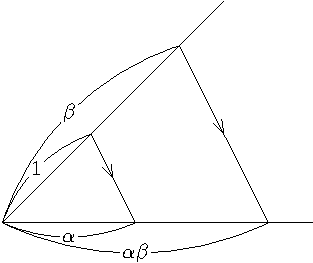
\includegraphics[height=5cm]{mult-crop.pdf}\end{center}
\end{frame}

\begin{frame}
また$\alpha \in L, \alpha > 0$なら$\sqrt{\alpha}$も$L$に属することが
分かる.

\begin{center}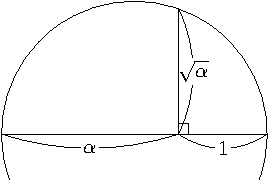
\includegraphics[height=4cm]{sqrt-crop.pdf}\end{center}
\end{frame}

\begin{frame}
また作図可能な点というのは直線と直線の交点,直線と円の交点,円と円の交点として現れる.

その座標は一次方程式,二次方程式の解であるので,結局,$L$は$0$と$1$から出発して和,差,積,商,平方根を有限回使って得られる実数全体となることがわかる.
\end{frame}

\begin{frame}
これを体の言葉で言い直すと次のようになる.

\begin{thm}
$\alpha \in \R$とするとき,次の条件(1), (2)は同値である.
\begin{enumerate}
\item $\alpha \in L$
\item 体の列$K_0 = \Q \subset K_1 \subset K_2 \subset \dots \subset K_n \subset \R$で$i = 1, \dots, n$に対し$\beta_i \in K_{i-1}$があり,$K_i = K_{i-1}(\sqrt{\beta_i})$となるものが存在し,$\alpha \in K_n$である.
\end{enumerate}
\end{thm}
\end{frame}

\begin{frame}
もっと短く言うと,$\alpha \in L$であるためには$\alpha$が$\Q$に$2$次拡大を積み上げた体に入っていることが必要十分である.
\end{frame}

\begin{frame}
例. たとえば作図可能な数
\[ \sqrt{2+\sqrt{3}} + \sqrt{5} \]
に対しては,次の体の列をとればよい.
\begin{align*}
\Q \subset \Q(\sqrt{3}) \subset \Q(\sqrt{3}, \sqrt{2+\sqrt{3}}) \\ 
\subset \Q(\sqrt{3}, \sqrt{2+\sqrt{3}}, \sqrt{5}) \end{align*}


\end{frame}

\begin{frame}
例. 正五角形は作図可能である.
\[ \cos \frac{2 \pi}{5} = \frac{-1 + \sqrt{5}}{4} \]
である.よって$\cos \frac{2 \pi}{5}$は作図可能.$\sin \theta = \sqrt{1 - \cos^2 \theta}$により$\sin \frac{2 \pi}{5}$も作図可能.よって点$(\cos \frac{2 \pi}{5}, \sin \frac{2 \pi}{5})$が作図可能なので正五角形は作図可能.
\end{frame}

\begin{frame}
\[ \cos \frac{2 \pi}{5} = \frac{-1 + \sqrt{5}}{4} \]
の証明.
$\zeta = \exp \frac{2 \pi i}{5}$とおくと,
\[ \zeta^4 + \zeta^3 + \zeta^2 + \zeta + 1 = 0 \]
である.
\end{frame}

\begin{frame}
\[ a = \zeta + \zeta^4, b = \zeta^2 + \zeta^3 \]
とおくと,
\[ a + b = -1, ab = -1. \]
よって$a, b$は2次方程式
\[ x^2 + x - 1 = 0 \]
の解.これを解くと
\[ x = \frac{-1 \pm \sqrt{5}}{2}. \]
\end{frame}

\begin{frame}
$a =  \zeta + \zeta^4 = \zeta + \zeta^{-1} = \zeta + \bar{\zeta} = 2 \mathrm{Re} \zeta = 2 \cos \frac{2 \pi}{5} $なので$a > 0$.よって,
\[a = \frac{-1 + \sqrt{5}}{2}.\]
したがって
\[\cos \frac{2 \pi}{5} = \frac{-1 + \sqrt{5}}{4}.\]
\end{frame}

\begin{frame}
これで表の$5$,$10$,$15$,$20$のところが○となる:
\small
\begin{table}[h]
  \begin{tabular}{ccccccccc}
    $n$ & $3$ & $4$ & $5$ & $6$ & $7$ & $8$ \\
    正$n$角形は作図可能 & ○ & ○ & \textcolor{red}{○} & ○ & ? & ○ \\
     & $9$ & $10$ & $11$ & $12$ & $13$ & $14$ \\
     & ? & \textcolor{red}{○} & ? & ○ & ? & ? \\
     & $15$ & $16$ & $17$ & $18$ & $19$ & $20$ \\
     & \textcolor{red}{○} & ○ & ? & ? & ? & \textcolor{red}{○}
  \end{tabular}
\end{table}
\end{frame}

\begin{frame}
補足:なぜ$15$が可能になるか?

\[\frac{2}{5} - \frac{1}{3} = \frac{1}{15}\]

に注意しよう.
\end{frame}

\begin{frame}
正$5$角形が作図可能なので一周の$2/5$の角が作図できて,正$3$角形が作図可能なので一周の$1/3$の角が作図可能になる.よってその二つの角の差であるところの一周の$1/15$の角も作図可能になるので正$15$角形が作図可能である.

%{\tiny ※ 一般に$m$と$n$が互いに素で正$m$角形と正$n$角形が作図可能なら正$mn$角形も作図可能}
\end{frame}

\begin{frame}
これから正$n$角形が作図可能であるための必要条件を考えよう.

$\zeta_n = \exp \frac{2 \pi i}{n}$とおく.

正$n$角形が作図可能だとすると$\Q$から$2$次拡大を重ねて得られる体$K$があり,$\cos \frac{2 \pi}{n} \in K$である.

拡大次数の積の法則より,$[\Q(\cos \frac{2 \pi}{n}) : \Q]$は$[K : \Q]$を割り切る.よって$[\Q(\cos \frac{2 \pi}{n}) : \Q]$は$2$べきである.

\end{frame}

\begin{frame}
ここで$[\Q(\zeta_n) : \Q(\cos \frac{2 \pi}{n})] = 2$である.

よって拡大次数の積の法則より$[\Q(\zeta_n) : \Q]$も$2$べきである.
\end{frame}

\begin{frame}
以上より,次の結果が得られた.

\begin{itemize}
\item 正$n$角形が作図可能 $\Rightarrow$ $[\Q(\zeta_n) : \Q]$は$2$べきである
\end{itemize}

この結果を得るのにガロア理論は使っていない.この結果の逆が成立するのだが,その証明にガロア理論を使う.

しかし,逆を証明する前に$[\Q(\zeta_n) : \Q]$は$2$べきであるという条件の必要十分条件を与えよう.
\end{frame}

\begin{frame}
$\zeta_n$の$\Q$上の最小多項式は次になることが知られている:
\[ \Phi_n(x) = \prod_{\substack{1 \le i \le n \\ \gcd(i, n) = 1}} (x - \zeta_n^i) \]
このことの証明は難しい.今は認めることにする.
\end{frame}

\begin{frame}
例.
\begin{align*}
\Phi_4(x) &= (x - \zeta_4)(x - \zeta_4^3) \\
&= (x - i)(x + i) = x^2 + 1
\end{align*}
\end{frame}

\begin{frame}
特に$\Phi_n(x)$の次数は
\[ \deg \Phi_n(x) = \phi(n) \]
である.ここに$\phi(n)$はオイラーの$\phi$関数で,$1 \le i \le n$で$\gcd(i, n) = 1$をみたす$i$の個数を表す.
\end{frame}

\begin{frame}
$\phi(n)$は次の性質をみたす (証明略).
\begin{itemize}
\item $m$と$n$が互いに素ならば$\phi(mn) = \phi(m)\phi(n)$
\item 素数$p$と整数$e \ge 1$について$\phi(p^e) = (p-1)p^{e-1}$
\end{itemize}
\end{frame}

\begin{frame}
では,$[\Q(\zeta_n) : \Q]$は$2$べきであるという条件の必要十分条件を与えよう.$\zeta_n$の$\Q$上の最小多項式が$\Phi_n(x)$なので
\[[\Q(\zeta_n) : \Q] = \deg \Phi_n(x) = \phi(n).\]
よって$\phi(n)$が$2$べきであることが必要十分.
\end{frame}

\begin{frame}
$n = 2^{e_0} p_1^{e_1} \dots p_r^{e_r}$と素因数分解するとき
\[\phi(n) = 2^{e_0 - 1} \prod_{i=1}^r (p_i - 1)p_i ^ {e_i - 1} \]
であるため,$\phi(n)$が$2$べきであるためには,各$i = 1, \dots, r$について$e_i = 1$かつ$p_i - 1$が$2$べきであることが必要十分.
\end{frame}

\begin{frame}
$p - 1$が$2$べきになる,つまり$p = 2^k + 1$と書ける奇素数には,フェルマー素数という名前がある.

よって,$[\Q(\zeta_n) : \Q]$は$2$べきであることは$n$を前スライドのように素因数分解するとき,すべての$i = 1, \dots, r$について$e_i = 1$かつ$p_i$がフェルマー素数であることが必要十分.
\end{frame}

\begin{frame}
以上で次が得られた:

正$n$角形が作図可能
\par  $\Downarrow$\par
$[\Q(\zeta_n) : \Q]$は$2$べきである
\par  $\Updownarrow$\par
$\phi(n)$は$2$べきである
\par  $\Updownarrow$\par
$n = 2^{e_0} p_1^{e_1} \dots p_r^{e_r}$と素因数分解するとき,すべての$i = 1, \dots, r$について$e_i = 1$かつ$p_i$がフェルマー素数であることが必要十分.	
\end{frame}

\begin{frame}
なお,フェルマー素数としては現在,次の$5$個が知られている:
\[3, 5, 17, 257, 65537.\]
これ以外にフェルマー素数が存在するかどうかは未解決問題である.
\end{frame}

\begin{frame}
以上で次の×がわかった
\small
\begin{table}[h]
  \begin{tabular}{ccccccccc}
    $n$ & $3$ & $4$ & $5$ & $6$ & $7$ & $8$ \\
    正$n$角形は作図可能 & ○ & ○ & ○ & ○ & \textcolor{red}{×} & ○ \\
     & $9$ & $10$ & $11$ & $12$ & $13$ & $14$ \\
     & \textcolor{red}{×} & ○ & \textcolor{red}{×} & ○ & \textcolor{red}{×} & \textcolor{red}{×} \\
     & $15$ & $16$ & $17$ & $18$ & $19$ & $20$ \\
     & ○ & ○ & ? & \textcolor{red}{×} & \textcolor{red}{×} & ○
  \end{tabular}
\end{table}
\end{frame}



\begin{frame}
では次の結果:
\begin{itemize}
\item 正$n$角形が作図可能 $\Rightarrow$ $[\Q(\zeta_n) : \Q]$は$2$べきである
\end{itemize}
の逆:
\begin{itemize}
\item $[\Q(\zeta_n) : \Q]$は$2$べきである $\Rightarrow$ 正$n$角形が作図可能
\end{itemize}
を示そう.
\end{frame}

\begin{frame}
$K = \Q(\zeta_n) \cap \R$とおく.

このとき$\cos \frac{2 \pi}{n} \in K$である.

$[\Q(\zeta_n) : \Q]$は$2$べきなので,拡大次数の積の法則から$[K : \Q]$も$2$べきである.

また,$\mathrm{Gal}(\Q(\zeta_n)/\Q)$がアーベル群なので,ガロアの基本定理により,$K/\Q$はガロア拡大で$\mathrm{Gal}(K/\Q)$は$\mathrm{Gal}(\Q(\zeta_n)/\Q)$の剰余群である.

よって,$\mathrm{Gal}(K/\Q)$も位数$2$べきのアーベル群である.
\end{frame}

\begin{frame}
よって有限アーベル群の基本定理により群の列
\[\mathrm{Gal}(K/\Q) = G_0 \supset G_1 \supset \dots \supset G_r = \{1\}\]
であって,$|G_i/G_{i+1}| = 2$であるものがある.
$\mathrm{Gal}(K/\Q)$の部分群$G_i$に対応する中間体を$M_i$とすると
\[\Q = M_0 \subset M_1 \subset \dots \subset M_r = K\]
であって,$[M_{i+1}:M_i] = 2$となる.
\end{frame}

\begin{frame}
したがって,$K$は$\Q$に$2$次拡大を積み上げた体である.

ゆえに$\cos \frac{2 \pi}{n} \in K$は作図可能.

よって正$n$角形は作図可能.
\end{frame}

\begin{frame}
以上より次の定理が得られた:
\begin{thm}
次の(1), (2), (3)は同値.
\begin{enumerate}
\item 正$n$角形が作図可能
\item $[\Q(\zeta_n) : \Q] = \phi(n)$は$2$べきである
\item $n = 2^{e_0} p_1^{e_1} \dots p_r^{e_r}$と素因数分解するとき
,すべての$i = 1, \dots, r$について$e_i = 1$かつ$p_i$がフェルマー素数である
\end{enumerate}
\end{thm}
\end{frame}

\begin{frame}
以上で表が埋まった
\small
\begin{table}[h]
  \begin{tabular}{ccccccccc}
    $n$ & $3$ & $4$ & $5$ & $6$ & $7$ & $8$ \\
    正$n$角形は作図可能 & ○ & ○ & ○ & ○ & × & ○ \\
     & $9$ & $10$ & $11$ & $12$ & $13$ & $14$ \\
     & × & ○ & × & ○ & × & × \\
     & $15$ & $16$ & $17$ & $18$ & $19$ & $20$ \\
     & ○ & ○ & \textcolor{red}{○} & × & × & ○
  \end{tabular}
\end{table}
\end{frame}

\begin{frame}
$3, 5, 17, 257, 65537$はフェルマー素数だったから正$257$角形,正$65537$角形も作図可能である

また,$2$べきと相異なるフェルマー素数の積で表せる$n$について正$n$角形が作図可能だったので$2040 = 2^3 \times 3 \times 5 \times 17$なども作図可能である.
\par \par
\footnotesize 	(2040年は1920年以来の作図可能な年です.そのときがきたら祝いましょう)
\end{frame}

\begin{frame}
ところで,この結果によれば$\cos \frac{2 \pi}{17}$は有理数から出発して四則演算と平方根を有限回使って書ける.実際それを書き下すとどうなるか.
\end{frame}

\begin{frame}
こうなる:
{\small 
\begin{align*}
\cos \frac{2 \pi}{17} = \frac{-1+\sqrt{17}}{16}+\frac{1}{8}\sqrt \frac{17-\sqrt {17}}{2}\qquad\qquad\qquad\\
+\frac{1}{4}\sqrt{\frac{17+3\sqrt{17}}{4}-\frac{1}{2}\sqrt \frac{17-\sqrt {17}}{2}-\frac{17+\sqrt {17}}{2}}.
\end{align*}}
\end{frame}

\begin{frame}{参考文献}

\begin{itemize}
\item 雪江明彦 (2010) 『代数学2 環と体とガロア理論』 日本評論社
\item 『数学セミナー 2016年9月号』日本評論社 特集=私の選ぶとっておきの数式 「正17角形の作図」(谷口隆)
\end{itemize}
\end{frame}

\end{document}